% !TeX root = ../full_report.tex

\chapter{State of the art}
\section{SIFT and bag-of-words}\label{sec:sift}
Until recently, the state of the art in image retrieval and matching
was based on the idea of
bag-of-words~\cite{philbin_object_2007,mikulik_learning_2013}.
The idea behind the approach is to represent an image as a histogram,
or collection of frequencies, of visual words. The visual words should
be small, representative patches of the images in the dataset.
Usually, these visual words are obtained in multiple steps. First,
local features are extracted and encoded. The most common feature used
is SIFT~\cite{lowe_distinctive_2004}, a 128-dimensional vector representing
scale-invariant features. Then, the features are extracted for all
images and clustered into clusters of similar features.
The representative for each cluster is the center of the cluster,
i.e. the mean of all features falling into that cluster.
Each image can then be represented as a histogram of the occurrences
of these representative features.
This histogram forms the image descriptor, which has as many dimensions
as there are representative features and clusters.

Finally, for image classification, a classifier can be learned from the
descriptors of all images in the dataset. On the other hand, for image
retrieval or matching, the descriptors can be directly matched against
each other, based on some similarity measure.
In both cases, it can be useful to project the descriptors into a Hilbert
space using a different similarity measure than euclidean distance
in the original descriptor space.
For classification, this is done by employing an SVM classifier with a
non-linear kernel~\cite{shawe-taylor_kernel_2004}.
Among the most popular kernels are the
radial basis function~\cite{scholkopf_comparing_1997}
and the chi-squared function~\cite{vedaldi_efficient_2012}.

Until recently, this approach has obtained state of the art results for
image retrieval tasks~\cite{mikulik_learning_2013}.

\section{Fisher vectors (FV)}\label{sec:fv}
The Fisher vector representation is based on the Fisher kernel, as described
by Jaakkola and Haussler~\cite{jaakkola_exploiting_1999}. The main idea
in their work is to derive a kernel function for discriminative classification,
where the kernel function is derived from a generative probability model.
For this, the log-likelihood with respect to a parameter $\log P(X|\theta)$
is considered, where $X$ is the data and $\theta$ the parameter.

The Fisher kernel is based on the gradient of this log-likelihood which
essentially captures how much the parameter contributes to the generation
of a sample $X$. This principle has been applied to images as well by
Sanchez et al.~\cite{sanchez_image_2013}, in the context of image
classification. Here, the data (or samples) are the local descriptors of
patches of images and the parameters to be estimated are the parameters
of a Gaussian Mixture Model (GMM) of these descriptors.
This means that we consider the descriptor of an image as a
combination of local descriptors, each being independent of all others,
with each local descriptor contributing to the global descriptor through
a GMM. This GMM can have any number
of parameters, which can be learned through the expectation maximization
algorithm. The Fisher vector is the gradient of the log-likelihood of this
GMM with respect to the parameters. Thus, it represents the combination
of deviations from the generative model of all local descriptors of the
image, for each parameter of the model.

Another important property is that the Fisher
vector embeds each local descriptor into a space of
different dimension, which consists of the weights, means and co-variances
of the Gaussians of the GMM. The dimensionality of the Fisher
vector is thus ultimately dependent on the number of Gaussians chosen for
the GMM.

It can be shown that this representation represents a kernel for a kernel
machine and can thus be used very efficiently by linear classifiers learning
their parameters in the Fisher kernel space.

While the Fisher vector representation has a high dimensionality, it
has been shown that it can be compressed efficiently
~\cite{sanchez_image_2013,perronnin_large-scale_2010} and could be applied
to large-scale image retrieval systems~\cite{perronnin_large-scale_2010}.

\section{VLAD}
Another important descriptor used in image retrieval systems is the
vector of locally aggregated descriptors or VLAD. It was introduced
by Jegou et al.~\cite{jegou_aggregating_2010} and is related to both
the bag-of-words and the Fisher vector representations described in
Sections~\ref{sec:sift}~and~\ref{sec:fv}.

As with the bag-of-words approach, a visual vocabulary is formed
using the k-means clustering algorithm. Then, for each visual
word $w$ (one of the $k$ centers of the output of k-means)
and each local descriptor $x$ associated with $w$ (where $w$ is the closest
center), the difference $x-w$ is added to the VLAD representing $w$.

Hence, VLAD is a sum over the differences between all local descriptors
and their associated visual word. This is similar to the Fisher vector
representation, which represents a sum of the deviations of local
descriptors from the generative model, which can be seen as consisting
of the visual vocabulary.

Jegou et al.~\cite{jegou_aggregating_2010} show that the VLAD representation
has many advantages over previous representations. For one, it achieves
state-of-the-art results on the Holidays dataset~\cite{jegou_hamming_2008}.
Furthermore, it can be compressed efficiently using principal component
analysis and still achieve promising results, making it much faster to
compute than the Fisher vector representation, even when compressed
as described in Section~\ref{sec:fv}.

\section{Deep learning with CNNs}
Starting with the results of AlexNet for image classification in the 2012
ImageNet challenge~\cite{krizhevsky_imagenet_2012,russakovsky_imagenet_2015},
image classification tasks have been dominated by CNNs, learned using
large amounts of data.

A general trend in image related tasks is to move to an end-to-end
approach, where the final objective is directly optimized using gradient
descent and the gradient is back-propagated to all previous parts of the
system. In contrast, the bag-of-words model requires a choice of
features (SIFT, ORB~\cite{rublee_orb:_2011}, \dots),
a choice of the method for clustering features (k-means),
a choice of the classifier (AdaBoost~\cite{freund_desicion-theoretic_1995},
SVM, \dots), as well as a choice of the kernel if an SVM classifier is used.

Using a CNN, features are extracted at a low abstraction level by the
first convolutional layers, then higher level features are formed
by combining low level features from the previous layers. Finally,
high-level features are combined into a classifier by linear layers.
The advantage of this approach is that the features are learned at all
abstraction levels. Furthermore, the modularity of the approach allows
us to easily transfer the lower level features learned from a large dataset
to a smaller dataset, where there may not be enough data to efficiently
learn lower level features.

The following sections describe the high-level architecture of the
most widely used CNNs in classification and image retrieval.
\subsection{AlexNet}
AlexNet~\cite{krizhevsky_imagenet_2012} contains five convolutional
layers and three linear layers. The first convolutional layer
has a large kernel and stride to quickly increase the receptive field
of the consequent filters. The first two convolutional layers are followed
by a pooling layer to further increase the receptive field.

Finally, an important improvement for AlexNet to avoid over-fit is
the addition of dropout layers~\cite{hinton_improving_2012} before the
two first linear layers.

Apart from that, AlexNet is a simple adaptation of LeNet by
LeCun et al.~\cite{lecun_gradient-based_1998} for the ImageNet challenge.

\subsection{VGG}
The VGG architecture, introduced by
Simonyan and Zisserman~\cite{simonyan_very_2014}
is the first to use exclusively $3\times3$ convolutional kernels.
This means that the receptive field of the
first filters is much smaller, and thus many more layers are needed,
as well as more pooling layers. The most popular VGG architectures
are VGG-16 and VGG-19, having 16 and 19 layers in total respectively.

Using smaller kernels in convolutions and consequently more layers
allows to reduce the number of trainable parameters used by the
network, while increasing the number of non-linear layers.
This was shown to allow better generalization properties, and thus less
over-fit~\cite{simonyan_very_2014}.

\subsection{ResNet, Inception, DenseNet}
The idea of increasing the number of layers is further developed
by the ResNet, DenseNet and Inception architectures. However,
naively increasing the number of layers leads to the problem of
vanishing gradient~\cite{hinton_fast_2006}.

All of these networks overcome the vanishing gradient problem by
introducing skip connections, where the output of a previous layer
is added to the output of a layer, skipping some number of layers in
between.

The ResNet architecture by He et al.~\cite{he_deep_2015} always uses blocks
of 3 layers along with a skip of those 3 layers. The smaller types of
ResNet use blocks of 2 layers.

The Inception architecture by Szegedy et al.~\cite{szegedy_inception-v4_2016}
uses a combination of skip connections of different length and different
types.

Finally, DenseNet by Huang et al.~\cite{huang_densely_2016} takes the
skip connection idea one step further:
the input of each layer is dependent on the output of all $n$ previous layers
to some extent.

Finally, all of the very deep architectures use batch norm layers to further
reduce over-fit: a batch norm layer simply normalizes the features over each
batch, and then applies a learnable scaling and shifting.

\section{Image retrieval using CNNs}
For image retrieval, the current state of the art is set by
Gordo et al.~\cite{gordo_deep_2016}. It is based on an
end-to-end approach. The goal is to learn a global descriptor for images
that is well suited for comparing images.

\begin{figure}
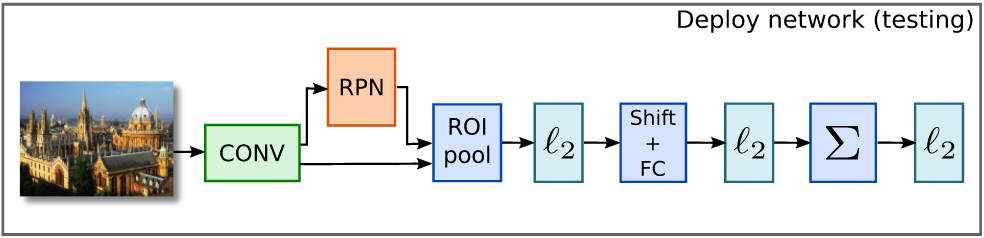
\includegraphics[width=\textwidth]{img/gordo_deepimageretrievaldeploy.png}
\caption{Architecture of a CNN network for image retrieval, developed by
Gordo et al.~\cite{gordo_deep_2016}
\label{fig:gordo_deploy}}
\end{figure}
Figure~\ref{fig:gordo_deploy} shows the detailed architecture used.
It first extracts the convolutional features of a pre-trained
CNN. Then, a Region Proposal Network (RPN)~\cite{ren_faster_2015} is
used to extract the regions of interest. For each region of interest,
a shifting and linear layer are used to reduce the dimensionality of
the descriptor. The final descriptor is simply a normalized sum of the
region-wise descriptors. This network can be learned end-to-end and
the obtained descriptor achieves state of the art results, which can
be even further improved by using query expansion and database side
feature augmentation (described in detail in Section~\ref{sec:improvedesc}).

Gordo et al.~\cite{gordo_deep_2016} found that using very deep networks
outperforms the shallower networks. The state of the art results are
thus set by a very deep ResNet architecture.

\subsection{Siamese networks and triplet loss}
\begin{figure}
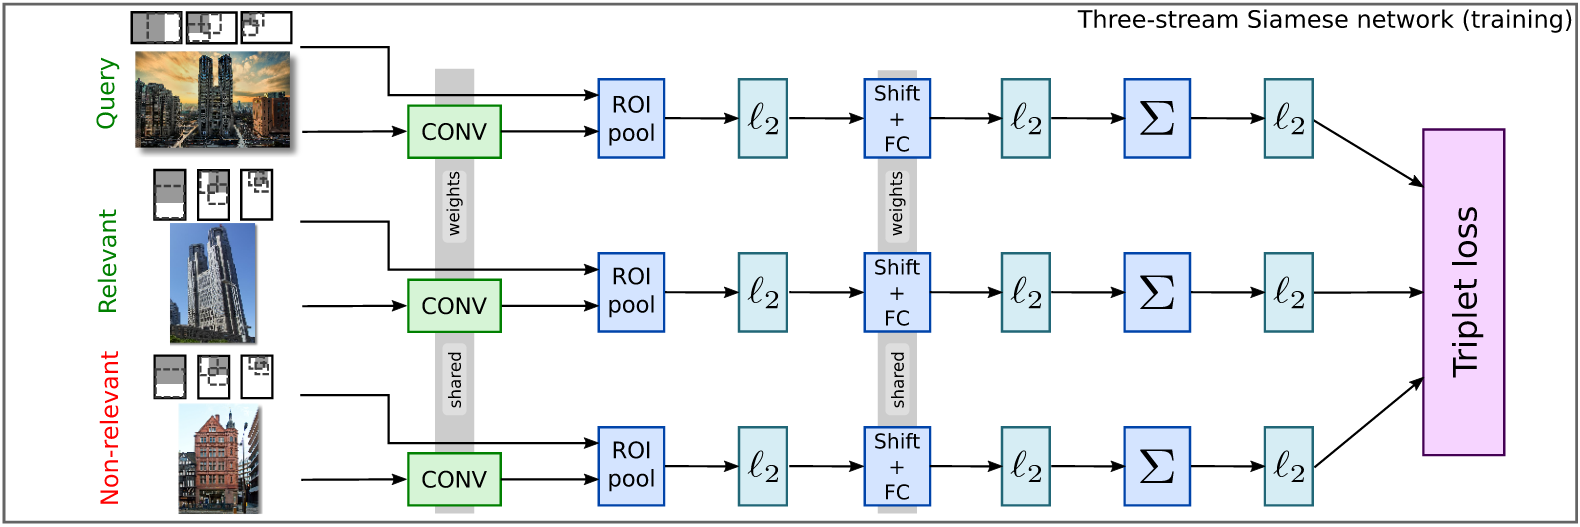
\includegraphics[width=\textwidth]{img/gordo_deepimageretrievalarc.png}
\caption{Siamese architecture of a CNN for image retrieval used in
training~\cite{gordo_deep_2016}
\label{fig:gordo_train}}
\end{figure}

Figure~\ref{fig:gordo_train} shows the architecture used to train the CNN
that produces a descriptor for images, as can be seen in
Figure~\ref{fig:gordo_deploy}.

The major difference is that during training, a Siamese architecture is
used: the CNN is evaluated with multiple images, using the same weights
for each. Then, a combined loss is obtained from the descriptors.
Finally, the loss is back-propagated once through all streams of the network,
since shared weights are used for all images.

In the case of this particular architecture, three images are evaluated
and a triplet loss is used. This triplet loss has previously been used
in face recognition tasks by Schroff et al.~\cite{schroff_facenet:_2015}.
The triplet loss was first introduced by
Weinberger et al.~\cite{weinberger_distance_2006} as a way of learning
the best suited distance metric in a k-nearest neighbor classification
problem. Section~\ref{sec:tripletloss} describes this loss in more detail.
This is the reason why the triplet loss was chosen for image retrieval:
the goal is to learn a metric which allows to discriminate couples of
images containing the same instance from couples of images containing
different instances, using the descriptors obtained from the Siamese
CNN.

Finally, Gordo et al. made further contributions, detailed in their
follow-up paper~\cite{gordo_end--end_2016}.
\subsection{Dataset}
For one, an important step is to use a suitable dataset. Datasets like
Oxford5k or Paris6k are too small for a network to learn a distance metric
applicable to any type of image. Instead, Gordo et al. use the much larger
Landmarks dataset, created by Babenko et al.~\cite{babenko_neural_2014}.
This dataset contains almost 200000 images in total of around 600
different landmarks, mostly buildings.

Another important step is the cleaning of the dataset. The Landmarks
dataset contains a lot of noise and weak labels: many images do not
represent the building they are labeled with. Gordo et al. use a meticulous
cleaning process: the main idea is to keep only the largest clusters
of matching objects for each of the landmarks. The implementation is
based on extracting SIFT and Hessian descriptors,
matching them and verifying matches with an affine transformation model.
This cleaning process is used in order to annotate the cleaned images
with regions of interest as well.

The cleaning requires a lot of processing,
but is only done once for the dataset.
The cleaned dataset is still fairly large, containing 49000 images and
586 instances of landmarks.

\subsection{Triplet choice}
Another important step is the choice of triplets during training of
the Siamese network. Schroff et al.~\cite{schroff_facenet:_2015}
and Weinberger et al.~\cite{weinberger_distance_2006} already identified
that using random triplets for training means that most triplets do not
contribute to the loss at all, thus leading to vanishing gradients.
So it makes sense to try and choose only the hardest triplets: for each
reference image, find the image with the same label that is furthest from the
reference image according to the current metric (the hardest positive),
and the closest from the reference image having a different label
(the hardest negative).
However, choosing the hardest positive and hardest negative at each step
is computationally too expensive.
So Schroff et al.~\cite{schroff_facenet:_2015}
propose choosing the hardest triplets for each batch. Since there are only
a few positive couples available in each batch, we simply choose all
positive couples along with the hardest negative for each reference image
in every batch. Since this can lead to a collapse in the model, Schroff
et al. propose choosing semi-hard negatives in the first epochs of
training: for each reference image and positive sample, choose the hardest
negative that is easier (further according to the metric) than the positive.

The disadvantage of this strategy is that it requires large batches.
Instead, Gordo et al.~\cite{gordo_end--end_2016} uses the following
strategy: pre-compute all descriptors in each epoch of training.
Then, for each reference image, choose the $n$ easiest positive samples
and the $m$ hardest negative samples. Compute the loss for all possible
combinations and use the $n$ hardest triplets, with highest loss.
This allows using smaller batches, while keeping the cost of computation
low, since descriptors are only computed every epoch. It may also help
eliminate some noise in the data, since only the easiest positive couples
are chosen.

\subsection{Limitations and goals}\label{sec:limitations}
The main limitation of Gordo's method is that it aims at producing a
general descriptor for comparing any type of image. This means that it
is most effective when trained on large datasets, with many samples
per instance. For datasets containing images from museums or tourist
sites, this is usually not applicable, as there are usually only very few
images available for each instance. While there are large datasets,
these datasets usually contain a large number of instances as well.
This makes it difficult to directly apply the state of the art on
our datasets.

On the other hand, it also means that the state of the art in
image retrieval wants to avoid over-fit at all costs:
the learned descriptor and metric should
be able to provide a good metric for any kind of image.
While this is usually desired in machine learning, in our case,
one goal is to provide a metric specifically designed
to discriminate between the images of the given dataset. This is because
an audio-guide in a museum can be fine-tuned for that museum, as long
as the fine-tuning is computationally cheap enough. So we do not care
if a given audio-guide cannot identify images of multiple museums,
as long as it can identify images of one museum with high precision.

Another limitation of the state of the art is that it requires
a tedious process to clean the dataset and annotate it with regions of
interest. This is not suited to museum datasets which are usually very
clean to begin with, by the nature of the dataset. Plus, the notion of
region of interest is usually not relevant for this type of image:
which part of a painting or piece of art contains the semantically
relevant information is not obvious.

Finally, an evaluation of the CNN developed by
Gordo et al.~\cite{gordo_deep_2016} was carried out.
We used the published weights obtained in training this CNN on the
Landmarks dataset.
Figure~\ref{fig:incorrectimg}
shows examples of images in our dataset that were correctly matched
with high confidence as well as images that were incorrectly matched.
From these images, we make the following observations in
Section~\ref{sec:incorrectimages}:

\begin{enumerate}
    \item Images that are very similar visually are well matched
    \item Images at different scales are not well matched
\end{enumerate}

Thus, a limitation of the current state of the art is matching
images, where the object of interest is at different scales.
